\subsection{Problem 18: Curve on a Sphere}

\begin{problem}
A curve $C$ spirals 3 times around the sphere centred at the origin and with radius 3, as shown below.

\vspace{0.5em}
\noindent
\begin{center}
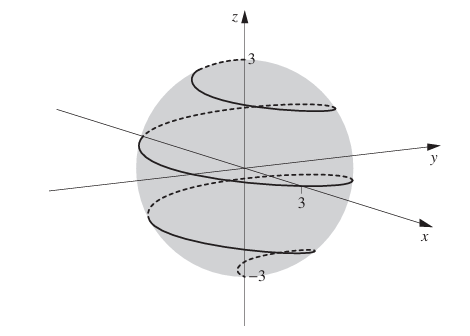
\includegraphics[width=0.6\textwidth]{images/18-01.png}
\end{center}
\vspace{0.3em}
\noindent\textit{Figure 1: Curve $C$ spiraling around the sphere}

\vspace{0.5em}
A particle is initially at the point $(0, 0, -3)$ and moves along the curve $C$ on the surface of the sphere, ending at the point $(0, 0, 3)$.

By using the diagram below, which shows the graphs of the functions $f(x)=\cos(\pi x)$ and $g(x)=\sqrt{9-x^{2}}$, and considering the graph $y=f(x)g(x)$, give a possible set of parametric equations that describe the curve $C$.

\vspace{0.5em}
\noindent
\begin{center}
\begin{tikzpicture}[scale=1.2, >=stealth]
    % Grid lines for reference (very thin)
    \draw[gray!15, very thin, step=1.0] (-4.5, -1.2) grid (4.5, 3.7);
    
    % Draw axes
    \draw[->, >=stealth, thick] (-4.5, 0) -- (4.5, 0) node[below right] {$x$};
    \draw[->, >=stealth, thick] (0, -1.2) -- (0, 3.7) node[above left] {$y$};
    
    % Draw tick marks on x-axis
    \foreach \x in {-4,-3,-2,-1,1,2,3,4} {
        \draw (\x, 0.1) -- (\x, -0.1) node[below, font=\small] {$\x$};
    }
    \node[below left, font=\small] at (0,0) {$O$};
    
    % Draw tick marks on y-axis
    \foreach \y in {-1,1,2,3} {
        \draw (0.1, \y) -- (-0.1, \y) node[left, font=\small] {$\y$};
    }
    
    % Plot g(x) = sqrt(9-x^2) as a red semicircle
    \draw[very thick, bookred] (3,0) arc (0:180:3);
    \node[bookred, above left] at (-1.6, 2.4) {$y = \sqrt{9-x^2}$};
    
    % Plot f(x) = cos(pi x) as a purple cosine curve
    \draw[very thick, bookpurple, samples=200, domain=-4:4] plot (\x, {cos(\x * 180)});
    \node[bookpurple, above right] at (3.1, 0.6) {$y = \cos(\pi x)$};
\end{tikzpicture}
\end{center}
\vspace{0.3em}
\noindent\textit{Figure 2: Graphs of $f(x)=\cos(\pi x)$ and $g(x)=\sqrt{9-x^{2}}$}
\end{problem}

\begin{hint}
The curve is on a sphere of radius 3, so $x^2 + y^2 + z^2 = 9$. The function $g(x) = \sqrt{9-x^2}$ suggests a relationship with the sphere. Use $f(x) = \cos(\pi x)$ to create the spiraling effect. Consider parameterizing with $t$ such that $z$ goes from $-3$ to $3$ as the parameter increases.
\end{hint}

